\documentclass[NormeDiProgetto.tex]{subfiles}
\begin{document}
\chapter{Processi primari}
\section{Fornitura}
In questa sezione vengono trattate le norme che i membri del gruppo \gruppo sono tenuti a rispettare al fine di proporsi e diventare fornitori nei confronti della Proponente Red Babel e dei committenti \Vardanega e \Cardin nell'ambito della progettazione, sviluppo e consegna del prodotto \progetto.


% TODO Rimuovere studio di fattibilità descrivendo cosa produrremo come grupo per la fine di questo periodo


\subsection{Studio di fattibilità}
In seguito alla presentazione ufficiale dei \textbf{Capitolati d'appalto} avvenuta Venerdì 10 novembre 2017 alle ore 10.30 presso l'aula 1C150 di Torre Archimede è stata convocata una riunione interna al gruppo per discutere in merito alla varie proposte presentate.\\
Una volta stabilita la scelta del capitolato per il quale proporsi come fornitori, gli analisti hanno condotto un'ulteriore e approfondita attività di analisi dei rischi e delle opportunità culminata con la redazione del documento \sdf \vruno. Tale documento include le motivazioni che hanno portato il gruppo \gruppo a proporsi come fornitore per il prodotto indicato e riporta per ciascun capitolato:
\begin{itemize}
	\item \textbf{Descrizione generale:} una sintesi del prodotto da sviluppare secondo quanto stabilito dal \citGloss{capitolato d'appalto};
	\item \textbf{Obbiettivo finale:} rappresenta il dominio Applicativo, cioè l'ambito di utilizzo del prodotto da sviluppare;
	\item \textbf{Tecnologie richieste:} rappresenta il dominio Tecnologico richiesto dal capitolato, raggruppando le tecnologie da impiegare nello sviluppo del progetto;
	\item \textbf{Valutazione finale:} racchiude le motivazioni, i rischi, le criticità evidenziate per le quali il capitolato in questione è stato respinto o accettato.
\end{itemize}

\section{Sviluppo}
\subsection{Analisi dei Requisiti}
L'analisi dei requisiti ha l'obbiettivo di individuare ed elencare tutti i \citGloss{requisiti} del capitolato. I requisiti possono essere estrapolati da più fonti:
\begin{itemize}
	\item \textbf{Capitolato d'appalto};
	\item \textbf{Verbali di riunioni esterne};
	\item \textbf{Casi d'uso}.
\end{itemize}
Il risultato di quest'analisi sarà il documento \adr \vruno redatto dagli \alisti, dopo essere stato verificato, al fine di:
\begin{itemize}
\item Descrivere l'obiettivo del lavoro del gruppo;
\item Fornire ai Progettisti riferimenti precisi ed affidabili;
\item Fissare le funzionalità e i \citGloss{requisiti} concordati col cliente;
\item Fornire una base per raffinamenti successivi al fine di garantire un
miglioramento continuo del prodotto e del processo di sviluppo;
\item Facilitare le revisioni del codice;
\item Fornire ai verificatori riferimenti per l'attività di test circa i casi d'uso principali e alternativi;
\item Stimare i costi.
\end{itemize}
Ogni requisito dovrà essere meno ambiguo possibile e rispettare le seguenti norme.

\subsubsection{Classificazione dei requisiti}
Ogni requisito è identificato da un codice, costruito come descritto di seguito:\\ \\
\textbf{\centerline{R[Importanza][Classificazione][Identificativo]}}\\
	\begin{itemize}
	\item La prima lettera (R) è l'abbreviazione di requisito;
	\item Il secondo valore indica l'\textbf{importanza}. Assume il valore:
		\begin{itemize}
				\item \textbf{Zero (0):} indica un requisito obbligatorio, il cui soddisfacimento
				dovrà necessariamente avvenire per garantire le funzioni base del
				sistema;
				\item \textbf{Uno (1):} se si tratta di un requisito desiderabile, cioè un requisito il cui
				soddisfacimento può dare maggiore completezza al sistema ma il
				non soddisfarlo non pregiudica alcuna funzione di base;
				\item \textbf{Due (2):} indica un requisito opzionale.
		\end{itemize}
	\item La terza lettera indica la \textbf{classificazione}. Assume valore F se si tratta di un Requisito funzionale, Q se di qualità, P se prestazionale e V se di vincolo;
	\item L'\textbf{identificativo} indica invece un numero progressivo.
	\end{itemize}

\subsubsection{Classificazione casi d'uso} Gli \alisti hanno anche il compito di identificare i casi d'uso, elencandoli con un grado di precisione che va dal generico verso il dettaglio. Ogni caso d'uso è descritto dalla seguente struttura:\\
\begin{itemize}
	\item \textbf{Codice identificativo e nome:} ogni caso d'uso è identificato da una serie di cifre separate dal punto. L'ultima cifra indica il numero del figlio, la penultima cifra indica il numero del padre e UC è l'abbreviazione di Use Case (caso d'uso in inglese). Queste cifre sono seguite dopo il trattino (-) dal nome del caso d'uso: \\\\
	\centerline{\textbf{UC[Codice padre].[Codice figlio] - Nome}}
	\item \textbf{Attori:} indica gli attori principali (ad esempio l'utente generico) e
	secondari (ad esempio ufficio universitario) del caso d'uso;
	\item \textbf{Scopo e descrizione:} riporta una breve descrizione del caso d'uso;
	\item \textbf{Scenario principale:} rappresenta il flusso degli eventi come lista
	numerata, specificando per ciascun evento il caso d'uso di riferimento;
	\item \textbf{Precondizione:} specifica le condizioni che sono identificate come vere
	prima del verificarsi degli eventi del caso d'uso;
	\item \textbf{Postcondizione:} specifica le condizioni che sono identificate come
	vere dopo il verificarsi degli eventi del caso d'uso;
	\item \textbf{Inclusioni (se presenti):} usate per non descrivere più volte lo stesso flusso di eventi,
	inserendo il comportamento comune in un caso d'uso a parte;
	\item \textbf{Estensioni (se presenti):} descrivono i casi d'uso che non fanno parte del flusso
	principale degli eventi, allo stesso modo di quanto descritto in “Scenario
	principale”.
\end{itemize}

\subsection{Progettazione}

\subsubsection{Scopo}
L'attività di Progettazione consiste nel descrivere una soluzione del problema
che sia soddisfacente per tutti gli stakeholders.
I \progi hanno il compito di svolgere tale attività, definendo l'architettura logica del prodotto identificando componenti chiare, riusabili e coese rimanendo nei costi fissati. La progettazione viene fatta in due momenti: una prima parte ad alto livello viene fatta durante il periodo di Progettazione della base tecnologica, dove verranno studiati i design pattern che potrebbero essere utilizzati durante il periodo seguente di Progettazione di dettaglio e codifica, durante il quale la progettazione diventa atomica per ogni componente del sistema, in modo che i \progri possano sviluppare il codice eseguendo task focalizzate e singolari.\\
L'architettura definita dovrà avere le seguenti qualità:
\begin{itemize}
	\item \textbf{Sufficienza:} deve soddisfare i \citGloss{requisiti} definiti nel documento \adr;
	\item \textbf{Comprensibilità:} affinchè possa essere capita dagli stakeholder;
	\item \textbf{Modularità:} deve essere suddivisa in parti chiare e ben distinte, così che possa essere facilmente manutenibile;
	\item \textbf{Robustezza:} deve essere capace di sopportare ingressi diversi, sia da parte di utenti che dall'ambiente;
	\item \textbf{Flessibilità:} deve poter permettere modifiche al variare o all'aggiunta di requisiti senza perdite di performance o doverla restaurare profondamente;
	\item \textbf{Riusabilità:} le sue parti devono poter essere usate in altre applicazioni;
	\item \textbf{Efficienza:} deve essere pensata in modo da poter ridurre gli sprechi di tempo e spazio;
	\item \textbf{Affidabilità:} deve avere una elevata capacità di rispettare le specifiche nel tempo;
	\item \textbf{Disponibilità:} la manutenzione delle sue parti non dovrà inabilitare il funzionamento di tutto il sistema;
	\item \textbf{Sicurezza:} rispetto ad intrusioni e malfunzionamenti;
	\item \textbf{Semplicità:} ogni parte contiene solo il necessario e nulla di superfluo;
	\item \textbf{Incapsulazione:} le componenti dovranno essere progettate in modo che le informazioni interne siano nascoste;
	\item \textbf{Coesione:} in modo che le parti che hanno gli stessi obiettivi stanno insieme;
	\item \textbf{Basso accoppiamento:} parti distinte devono essere poco dipendenti l'una dalle altre, in modo da poter essere facilmente manutenibili.
\end{itemize}
%TODO questa parte sotto la teniamo o è un po' ripetitiva?
\subsubsection{Obiettivi della progettazione}
Essa serve a garantire che il prodotto sviluppato soddisfi le proprietà e i bisogni specificati nell'attività di analisi ponendo i seguenti obiettivi:
\begin{itemize}
	\item Garantire la qualità di prodotto sviluppato, perseguendo la \textit{correttezza per costruzione};
	\item Organizzare e ripartire compiti implementativi, riducendo la
	complessità del problema originale fino alle singole componenti
	facilitandone la codifica da parte dei singoli \progri;
	\item Rendere chiara e comprensibile ogni parte dell'architettura ai differenti stakeholders;
	\item Mantenere nascosti i dettagli implementativi, seguendo il principio dell'\textit{information hiding};
	\item Mantenere bassa la dipendenza tra le varie parti del prodotto, seguendo il principio della \textit{modularità};
	\item Ottimizzare l'uso di risorse.
\end{itemize}
%TODO fino a qua
\subsubsection{Diagrammi}
Al fine di rendere più chiare le scelte progettuali adottate e
ridurre le possibili ambiguità, sarà necessario fare largo uso di vari tipi di diagrammi 
\textbf{UML 2.0}, realizzandone secondo le seguenti rappresentazioni:
\begin{itemize}
	\item \textbf{Diagrammi dei casi d'uso:} dedicati alla descrizione delle funzioni offerte dal sistema;
	\item \textbf{Diagrammi delle classi:} dedicati alla descrizione degli oggetti che fanno parte di un sistema e delle loro dipendenze;
	\item \textbf{Diagrammi dei package:} dedicati alla descrizione della dipendenza tra classi raggruppate in package;
	\item \textbf{Diagrammi di sequenza:} dedicati a descrivere la collaborazione nel tempo tra un gruppo di oggetti;
	\item \textbf{Diagrammi di attività:} dedicati a descrivere la logica procedurale.
\end{itemize}
Per svolgere al meglio il processo di progettazione, viene utilizzato il software PlantUML\footnote{\nURI{http://plantuml.com/}}, che permette di creare diagrammi UML in maniera semplice e veloce. Infatti mette a disposizione strumenti adatti per creare tutti i tipi di diagrammi utili alla progettazione, come i diagrammi delle classi, di sequenza e di attività.

\subsubsection{Diagrammi delle classi}
Lo scopo dei diagrammi delle classi può essere sintetizzato in:
\begin{itemize}
	\item Analisi e progettazione della visione statica di un'applicazione;
	\item Descrizione delle responsabilità di un sistema;
	\item Base per diagrammi dei componenti e di rilascio;
	\item Ingegneria diretta e inversa.
\end{itemize}
Per creare facilmente i diagrammi delle classi, deve essere creato un file per ogni classe o raggruppamento di classi che dovrà avere estensione \texttt{.iuml}. In questo modo saranno più facilmente manutenibili e modificabili.\\
Per stabilire le relazioni tra le classi viene creato un'altro file con estensione \texttt{.puml} in modo da avere il diagramma completo.
\paragraph{React}
Ogni componente React viene rappresentato attraverso un rettangolo tripartito orizzontalmente, così suddiviso:
\begin{enumerate}
	\item \textbf{Nome componente:} deve essere univoco, scritto seguendo la notazione \citGloss{CamelCase}, in inglese;
	\item \textbf{Props:} se presenti, devono essere elencate seguendo la notazione
	\begin{center}
		\texttt{propName : type};
	\end{center}
	\item \textbf{Render:} breve descrizione della renderizzazione del componente.
\end{enumerate}
I componenti di routing vengono invece rappresentati attraverso un rettangolo bipartito orizzontalmente. La prima sezione è sempre occupata dal nome seguendo le norme valide per i componenti React, mentre la seconda sezione elenca le routes.

\paragraph{Redux}
Le \citGloss{Sagas} e i \citGloss{Ducks} Redux sono rappresentati attraverso un rettangolo diviso orizzontalmente in quattro sezioni:
\begin{enumerate}
	\item \textbf{Nome saga/duck:} deve essere univoco, scritto seguendo la notazione \citGloss{CamelCase}, in inglese;
	\item \textbf{Types:} deve elencare la lista secondo la notazione 
	\begin{center}
		\texttt{modifier NAME\_TYPE : type};
	\end{center}
	\item \textbf{Sagas/Selectors:} elenca la lista di metodi secondo la notazione 
	\begin{center}
		\texttt{modifier methodName( parameterTypes ) : returnType};
	\end{center}
	\item \textbf{Actions:} elenca la lista delle azioni secondo la notazione 
	\begin{center}
		\texttt{modifier methodName( parameterTypes ) : returnType}.
	\end{center}
\end{enumerate}
Ogni membro del duck dovrà inserire obbligatoriamente il modificatore d'accesso e deve essere uno di questa lista:
\begin{itemize}
	\item +: visibilità pubblica;
	\item -: visibilità privata;
	\item *: per indicare funzioni di tipo \texttt{generators}.
\end{itemize}
Ogni Duck dovrà essere accompagnato da una nota che indichi lo stato iniziale secondo la notazione
\begin{center}
	\texttt{initialState: \{name : type = default\}}
\end{center}
Le interfacce vengono rappresentate con un rettangolo tripartito orizzontalmente così suddiviso:
\begin{enumerate}
	\item \textbf{Nome interfaccia:} deve essere univoco, scritto seguendo la notazione \citGloss{CamelCase}, in inglese;
	\item \textbf{Metodi:} 	
	\begin{center}
		\texttt{modifier methodName( parameterTypes ) : returnType}.
	\end{center}
	\item \textbf{Purpouse:} piccola descrizione dell'interfaccia.
\end{enumerate}
I modificatori antecedenti ai nomi 

\paragraph{Solidity}
I contratti in Solidity vengono rappresentati con un rettangolo suddiviso in quattro parti orizzontalmente così descritto:
\begin{enumerate}
	\item \textbf{Nome contratto:} deve essere univoco, scritto seguendo la notazione \citGloss{CamelCase}, in inglese;
	\item \textbf{Campi dati:} elenco dei campi dati del contratto, secondo la notazione: \texttt{modifier name : type}. Il modificatore d'accesso dovrà essere obbligatoriamente inserito e deve essere uno di questi:
	\begin{itemize}
		\item +: visibilità pubblica;
		\item \textendash: visibilità privata;
		\item \#: visibilità interna;
	\end{itemize}
	\item \textbf{Modifiers:} elenco dei modificatori di quel contratto, secondo la notazione:
		\texttt{modifierName( value : type )};
	\item \textbf{Metodi:} elenco dei metodi del contratto, secondo la notazione:
	\begin{center}
		\texttt{modifier methodName( value : type ) : type}
	\end{center}
	e il modificatore d'accesso dovrà essere obbligatoriamente inserito, e oltre a quelli utilizzabili per i campi dati, può essere utilizzato contemporaneamente anche il simbolo \texttt{@} per indicare che si tratta di una \texttt{view}.
\end{enumerate}

Per tutti i linguaggi, nel caso in cui una classe non dovesse possedere variabili e/o metodi, apparirà nel diagramma comunque, seppur vuota, la sezione ad esse dedicata.

I diagrammi delle classi sono collegati fra loro da frecce che esplicitano le dipendenze.
In particolare, verranno utilizzati i seguenti tipi di freccia:
\begin{itemize}
	\item Freccia semplice, da classe A a classe B: indica che la classe A ha fra i propri campi dati una o più istanze della classe B;
	\begin{figure}[h]
		\centering
		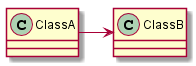
\includegraphics[width=0.4\linewidth]{progettazione/dip}
		\caption{Relazione di dipendenza forte in diagramma delle classi.}
		\label{fig:dip}
	\end{figure}
	\newpage
	\item Freccia tratteggiata, da classe A a classe B: indica una dipendenza, significa che A dipende da B secondo una primitiva che andrà esplicitata vicino alla freccia;
	\begin{figure}[h]
		\centering
		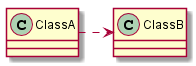
\includegraphics[width=0.4\linewidth]{progettazione/dipdebole}
		\caption{Relazione di dipendenza debole in diagramma delle classi.}
		\label{fig:dipdebole}
	\end{figure}
	
	\item Freccia a diamante vuota, da classe A a classe B: indica un'aggregazione, una relazione non forte ovvero una relazione nella quale le classi parte hanno un significato anche senza che sia presente la classe tutto;
	\begin{figure}[h]
		\centering
		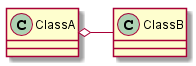
\includegraphics[width=0.4\linewidth]{progettazione/aggreg}
		\caption{Relazione di aggregazione in diagramma delle classi.}
		\label{fig:aggreg}
	\end{figure}
	
	\item Freccia a diamante piena, da classe A a classe B: indica la composizione, definita come una relazione forte cioè una relazione nella quale le classi parte hanno un reale significato solo se sono legate alla classe tutto;
	\begin{figure}[h]
		\centering
		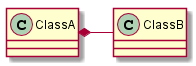
\includegraphics[width=0.4\linewidth]{progettazione/compos}
		\caption{Relazione di composizione in diagramma delle classi.}
		\label{fig:compos}
	\end{figure}
	
	\item Freccia vuota, da classe A a classe B: indica l'ereditarietà/generalizzazione ed è il massimo grado di dipendenza fra classi. Indica che ogni oggetto di A è anche un oggetto di B.
	\begin{figure}[h]
		\centering
		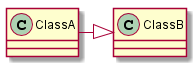
\includegraphics[width=0.4\linewidth]{progettazione/ered}
		\caption{Relazione di ereditarietà in diagramma delle classi.}
		\label{fig:ered}
	\end{figure}
	
\end{itemize}
\newpage
\subsubsection{Diagramma dei package}
Ogni package verrà rappresentato tramite un rettangolo con un'etichetta per il nome, che dovrà contenere i diagrammi delle classi appartenenti al package ed eventuali sotto-package. Le dipendenze fra i vari package dovranno essere segnalate con una freccia tratteggiata. Tale freccia, disegnata dal package A al package B, indica una dipendenza di A ne confronti di B.
\begin{figure}[h]
	\centering
	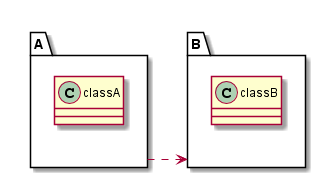
\includegraphics[width=0.4\linewidth]{progettazione/package}
	\caption{Relazione di dipendenza di package.}
	\label{fig:package}
\end{figure}

\subsubsection{Diagrammi di sequenza}
Ogni diagramma di sequenza avrà un senso di lettura verticale dall'alto al basso (verso che indica lo scorrere del tempo). Gli oggetti coinvolti verranno rappresentati tramite un rettangolo, al cui interno si troverà un nome per identificarli nel formato istanza: NomeClasse. Sotto ad ogni istanza si troverà una linea della vita tratteggiata, che sarà sormontata in alcuni tratti da una barra di attivazione che indica i momenti in cui l'oggetto e attivo. Da una barra di attivazione partiranno delle frecce, che rappresentano un messaggio/segnale, verso la linea della vita di oggetti già instanziati o, in alternativa, verso una nuova istanza di classe per crearla. In particolare, verranno utilizzati i seguenti tipi di frecce:
\begin{itemize}
\item  Freccia piena, per indicare un messaggio sincrono: corrisponde alla chiamata di un
metodo. Sopra tale freccia si dovrà specificare il metodo invocato secondo il formato
nomeMetodo(lista parametri formali);
\item  Freccia, per indicare un messaggio asincrono (chi invoca il metodo non attende il
return);
\item  Freccia tratteggiata, per indicare il ritorno di un metodo chiamato. Sopra tale
freccia si dovrà indicare il tipo di ritorno secondo il formato TipoRitorno;
\item  Freccia tratteggiata sormontata da <<create>>, indica la creazione di un nuovo
oggetto e termina sempre in un rettangolo che ne contiene il nome nel formato
istanza: NomeClasse;
\item  Freccia piena sormontata da <<destroy>>, indica la distruzione di un oggetto e
termina sempre in una X, nella quale muore anche la linea della vita dell'oggetto.
\end{itemize}
Sarà inoltre possibile determinare sui diagrammi di sequenza dei frame di interazione associati ad una guardia (o condizione):
\begin{itemize}
\item  alt: indica dei frammenti in alternativa fra loro, verrà eseguito quello per cui la guardia è verificata;
\item  opt: indica un frammento che viene eseguito solo se la guardia è specificata;
\item  par: indica frammenti eseguiti in parallelo;
\item  loop: indica un frammento che viene eseguito più volte, la condizione di arresto del ciclo è la guardia;
\item region: indica un frammento critico che deve essere eseguito in mutua esclusione.
\end{itemize}

\subsubsection{Diagrammi di attività}
I diagrammi delle attività conterranno, collegati sempre da frecce, i seguenti elementi, che verranno indicati con i formalismi indicati:
\begin{itemize}
\item  Nodo iniziale, rappresentato da un pallino pieno. \'E il punto da cui inizia l'esecuzione. Genera un token;
\item  Activity, rappresentata da un rettangolo che ne contiene la descrizione. La descrizione dovrà essere il più breve e concisa possibile, è possibile una sintassi sincopata della frase, composta per lo più da parole chiave. Consuma e produce un token;
\item Subactivity, rappresentata da un rettangolo che ne contiene il nome (sempre indicato con la lettera maiuscola) e un piccolo tridente nell'angolo in basso a destra. \'E un riferimento ad una sottoattività il cui diagramma viene descritto separatamente. Ogni sottoattività ha un input ed un output;
\item Branch, rappresentato da un rombo con una freccia in ingresso e n in uscita. \'E
un punto in cui si può prendere solo uno degli n rami, ognuno dei quali deve avere
scritta in prossimità la guardia, secondo il formato [guardia]. Consuma e produce
un token;
\item Merge, rappresentato da un rombo con n frecce in ingresso e una in uscita. \'E
un punto in cui gli n rami generati da un Branch tornano ad unirsi. Consuma e produce un token;
\item Fork, rappresentato da una linea lunga orizzontale o verticale. \'E un punto in cui l'attività si parallelizza senza vincoli di esecuzione temporale, ha una freccia in ingresso e n in uscita. Consuma un token e ne genera n;
\item Join, rappresentato da una linea lunga orizzontale o verticale. \'E un punto in cui avviene la sincronizzazione fra processi paralleli, ha n frecce in ingresso e una in uscita. Consuma n token e ne genera uno;
\item Pin, rappresentato da un piccolo quadratino dove entrano/escono frecce dalle Activity. Indica il passaggio di un parametro, il cui tipo va indicato di fianco secondo il formato TipoParametro;
\item Segnali, rappresentati da due figure a incastro, la prima (non bloccante) per
l'emissione del segnale, la seconda (bloccante) per la ricezione dello stesso. Al loro
interno devono contenere <<signal sending>> o <<signal receipt>>, seguiti da una
descrizione breve e concisa con sintassi sincopata;
\item Timeout, rappresentato da una clessidra, serve per modellare timeout o eventi ripetuti. I timeout hanno frecce entranti e frecce uscenti, al contrario degli eventi ripetuti che possono avere solo archi uscenti. Di fianco devono avere una descrizione così composta: i timeout devono cominciare con "wait" e le azioni ripetute con "every", di seguito dovrà trovarsi un indicazione temporale o una descrizione in linguaggio naturale breve e concisa;
\item Nodo di fine flusso, rappresentato da un cerchio vuoto con una X al centro. \'E
un punto in cui uno dei rami di esecuzione va a morire, ma l'esecuzione continua comunque sugli altri rami paralleli. Consuma un token;
\item Nodo finale, rappresentato da due cerchi concentrici di cui il più esterno vuoto e il più interno pieno. \'E il punto da cui termina l'esecuzione. Consuma un token.

\subsubsection{Sviluppo}
Lo sviluppo di \progetto avviene seguendo il modello incrementale, spiegato nel dettaglio nel documento \pdp \S 3. Sarà eseguita un'analisi comparativa di varie tecnologie esistenti al fine di capire quali siano le più consone allo sviluppo di \progetto. Nel caso si ritengano più consone tecnologie differenti da quelle proposte dalla proponente, il gruppo \gruppo la contatterà per discuterne insieme.\\
La proponente, tramite capitolato d'appalto, identifica queste tecnologie come obbligatorie per lo sviluppo:\\
\begin{itemize}
	\item \textbf{\citGloss{React};}
	\item \textbf{\citGloss{Redux};}
	\item \textbf{\citGloss{Metamask};}
	\item \textbf{Rete \citGloss{Ethereum}.}
\end{itemize}

\subsubsection{Integrazione}
L'attività di integrazione sarà effettuata utilizzando il servizio, compatibile con \citGloss{GitHub}, \textit{\citGloss{Travis}}.\\
Questo servizio implementa il modello di integrazione continua: ad ogni commit su repository \citGloss{GitHub}, \citGloss{Travis} crea una build ed esegue automaticamente i test di unità. In questo modo sarà possibile identificare immediatamente modifiche od errori che inficiano sul comportamento del prodotto.\\
Per quanto riguarda il test coverage, cioè il grado di esecuzione del codice sorgente durante l'esecuzione dei test, verrà utilizzato il tool \citGloss{JavaScript} \textit{IstanbulJS}. 

\subsection{Codifica}
In questa sotto-sezione vengono elencate le norme alle quali i \progri devono attenersi durante l'attività di programmazione e implementazione.\\
All'inizio verranno elencate delle norme generali a cui i \progri devono attenersi con qualsiasi linguaggio di programmazione utilizzato, mentre di seguito verranno elencate delle norme specifiche per i linguaggi \citGloss{JavaScript}, \citGloss{JavaScript} Syntax eXtension, Solidity e \citGloss{SCSS}.\\
Ogni norma è rappresentata da un paragrafo; ciascuna ha un titolo, una breve descrizione e, se necessario, un esempio che illustri le convenzioni da applicare. Alcune di esse includono inoltre una lista di possibili eccezioni d'uso.\\
L'uso di norme e convenzioni è fondamentale per permettere la generazione di codice leggibile e uniforme, agevolando così le fasi di manutenzione, \citGloss{verifica} e \citGloss{validazione} e migliorando la qualità del prodotto.

\paragraph*{Convenzioni per i nomi: }
\begin{itemize}
	\item Alcuni nomi sono da evitare in quanto facilmente confondibili con i numeri \texttt{1} e \texttt{0}, elencati di seguito:
	\begin{itemize}
		\item \texttt{l} (lettera minuscola elle);
		\item \texttt{O} (lettera maiuscola o);
		\item \texttt{I} (lettera maiuscola i).
	\end{itemize}
	\item Tutti i nomi devono essere \textbf{unici} ed \textbf{esplicativi} al fine di evitare al più possibile ambiguità e comprensione.
\end{itemize}
Per i vari linguaggi verranno successivamente descritte altre norme per nomi di variabili, funzioni e altro facendo riferimento ai seguenti stili:
\begin{itemize}
	\item \texttt{lowercase};
	\item \texttt{lower\_case\_with\_underscores};
	\item \texttt{UPPERCASE};
	\item \texttt{UPPER\_CASE\_WITH\_UNDERSCORES};
	\item \texttt{CapitalizedWords} (o \texttt{CapWords});
	\item \texttt{mixedCase};
	\item \texttt{Capitalized\_Words\_With\_Underscores};
	\item \texttt{lower-case-with-dashes}.
\end{itemize}

\paragraph*{Convenzioni per la documentazione: }
\begin{itemize}
	\item Tutti i nomi e i commenti al codice per la documentazione vanno scritti in \textbf{inglese};
	\item \`{E} possibile utilizzare in un commento la keyword \textbf{TODO} per indicare codice temporaneo e soluzioni a breve termine o evidentemente migliorabili;
	\item Ogni file contenente codice deve avere la seguente \textbf{intestazione} contenuta in un commento e posta all'inizio del file stesso:
\begin{center}{
\begin{minipage}{12cm}
\begin{Verbatim}[frame=single]
File : nome file
Version : versione file
Type : tipo file
Date : data di creazione
Author : nome autore/i
E- mail : email autore/i

License : tipo licenza

Advice : lista avvertenze e limitazioni

Changelog :
Autore || Data || breve descrizione delle modifiche
\end{Verbatim}
\end{minipage}
}
\end{center}
	\item La \textbf{versione} del codice viene inserita all'interno dell'intestazione del file e rispetta il
	seguente formalismo:
	\begin{center}{\textbf{X.Y}}\end{center}	
	\begin{itemize}
		\item \textbf{X}: è l'indice di versione principale, un incremento di tale indice rappresenta un avanzamento della versione stabile, che porta il valore dell'indice Y ad essere azzerato;
		\item \textbf{Y}: è l'indice di modifica parziale, un incremento di tale indice rappresenta una \citGloss{verifica} o una modifica rilevante, come per esempio la rimozione o l'aggiunta di una istruzione.
	\end{itemize}
	La versione \textit{1.0} deve rappresentare la prima versione del file completo e stabile, cioè quando le sue funzionalità obbligatorie sono state definite e si considerano funzionanti. Solo dalla versione \textit{1.0} è possibile testare il file, con degli appositi test predefiniti, per validarne la qualità.
\end{itemize}


\subfile{Codifica/Javascript.tex}
\subfile{Codifica/React.tex}
\subfile{Codifica/Solidity.tex}
\subfile{Codifica/Scss.tex}


\subsection{Procedure}

\subsubsection{Tracciamento componenti-requisiti}
	Si è scelto di utilizzare il software \citGloss{Trender} per il tracciamento automatizzato di tutte le informazioni ricavate dall'analisi dei \citGloss{requisiti}.\\
	Il database MySQL che garantisce la persistenza e l'accesso ai dati si trova su un server remoto, in modo tale da rendere sempre disponibile a tutti le informazioni che esso contiene.\\
	Qualsiasi componente del gruppo, utilizzando la parte \citGloss{front-end} dell'applicazione scritta in PHP e \citGloss{JavaScript}, può accedervi utilizzando l'account comune predisposto.\\
	Una volta effettuato l'accesso si ha a disposizione le funzionalità di modifica e di esportazione in codice \citGloss{LaTeX} dei dati presenti.\\
	
	%VERI_GIORAT aggiunta di Diagramma tracciamento componenti requisiti per rimpiazzare paragrafo precedente.
	
%	\citGloss{Trender} consente di mantenere il tracciamento di:\\
%	\begin{itemize}
%		\item \citGloss{requisiti};
%		\item Casi d'uso;
%		\item Attori;
%		\item Verbali;
%		\item Package;
%		\item Classi;
%		\item Test;
%		\item Voci del glossario.
%	\end{itemize}

\subsection{Strumenti}
Gli elementi indicati con \textbf{*} sono stati analizzati per l'utilizzo nelle fasi successive del progetto ma potrebbero essere cambiati in caso di necessità differenti da quanto pianificato.
\begin{itemize}
	\item \textbf{Tracciamento requisiti:} il gruppo \gruppo ha deciso di utilizzare il software \textbf{Trender}\footnote{\nURI{https://github.com/campagna91/Trender}} installato su server remoto condiviso;
	\item \textbf{Creazione diagrammi UML:} {UML Designer}\footnote{\nURI{http://www.umldesigner.org/}};
	\item \textbf{Scrittura del codice:} Webstorm by Jetbrains\footnote{\nURI{https://www.jetbrains.com/webstorm/}} per \citGloss{JavaScript} e Visual Studio Code\footnote{\nURI{https://code.visualstudio.com/}} per \citGloss{Solidity}; 
	\item \textbf{Toolkit sviluppo:} si utilizzano i pacchetti installabili tramite Node.js con gestore di pacchetti npm per risolvere dipendenze delle librerie e tool richiesti;
	\item \textbf{Esecuzione dei test:}
	\begin{itemize}
		\item \citGloss{React}: Mocha\footnote{\nURI{https://github.com/mochajs/mocha}}, Chai\footnote{\nURI{http://chaijs.com/}} e Enzyme\footnote{\nURI{https://github.com/airbnb/enzyme}};
		\item \citGloss{Redux}: Mocha e Chai;
		\item \citGloss{Solidity}: Mocha e Chai.
	\end{itemize}
	\item \textbf{Continuous Integration:} Travis\footnote{\nURI{http://travis-ci.com/}};
	\item \textbf{Tracciamento e copertura dei test:} 
	\begin{itemize}
		\item \textbf{Generazione copertura React e Redux:} Istanbul.JS \footnote{\nURI{https://istanbul.js.org}};
		\item \textbf{Generazione copertura Solidity:} Solidity-Coverage\footnote{\nURI{https://github.com/sc-forks/solidity-coverage}};
		\item \textbf{Visione online copertura test:} Codeclimate\footnote{\nURI{https://codeclimate.com/}}.
	\end{itemize}
	\item \textbf{Tool di supporto:} Scss-lint\footnote{\nURI{https://github.com/brigade/scss-lint}}. 	
\end{itemize}


\end{document}